\hide{
	
	\begin{table*}
		\newcolumntype{?}{!{\vrule width 0.5pt}}
		\newcolumntype{C}{>{\centering\arraybackslash}m{3em}}
		\caption{
			\label{tb:domain_adaptation} Performance (\%) of Anomaly Detection in the Supervised Setting.
		}
		\centering 
		\renewcommand\arraystretch{1.0}
		\begin{tabular}{@{~}c?@{~}*{1}{C??}*{1}{C?}*{1}{C?}*{1}{C?}*{1}{C??}*{1}{C?}*{1}{C?}*{1}{C?}*{1}{C??}*{1}{C}@{~}}
			\toprule
			
			
			%\diagbox{Datasets}{Methods}
			
			&{\textbf{Metrics}} &{\textbf{GCN}} &{\textbf{GAT}} &{\textbf{\tabincell{c}{Graph-\\SAGE}}} &{\textbf{GIN}} &{\textbf{\tabincell{c}{Logist-\\Reg}}} &{\textbf{\tabincell{c}{Genin-\\Path}}} &{\textbf{\tabincell{c}{Graph-\\Consis}}} &{\textbf{\tabincell{c}{CARE-\\GCN}}} 
			&{\textbf{\model}}
			\\
			\bottomrule
			\multirow{2}{*}[-0.5ex]{\textbf{AMiner}} 	
			&  AUC  & 75.68 & 74.97 & 73.01 & 74.28 & 62.49 & 76.18 & 68.89 & 77.64 &\textbf{88.07}\\
			\cmidrule{2-11}
			&   MAP & 59.28 & 59.87 & 60.51 & 57.75 & 33.68 & 50.67 & 50.11 & 55.18 &\textbf{76.02}\\
			\bottomrule
			%\bottomrule
			
			
			\multirow{2}{*}[-0.5ex]{\textbf{MAS}} 	
			&  AUC & 78.44 & 80.25 &  80.81 & 75.62 & 73.67 &81.93 & 74.98& 80.33& \textbf{87.52}\\
			\cmidrule{2-11}
			&   MAP & 63.89 & 62.75 & 68.74& 59.96 & 56.64& 65.66& 56.81 & 67.15& \textbf{72.75}\\
			
			\bottomrule
			%\bottomrule
			\multirow{2}{*}[-0.5ex]{\textbf{Alpha}} 	
			&  AUC & 82.12 & 78.45& 79.23 & 87.39 & 71.88 & 75.02 & 86.99 & 84.26 & \textbf{89.31}\\
			\cmidrule{2-11}
			&   MAP & 78.09 & 76.32 & 75.14 & 86.79 & 72.43 & 68.89 & 86.33 & 85.20 & \textbf{88.17}\\
			
			\bottomrule
			%\bottomrule
			\multirow{2}{*}[-0.5ex]{\textbf{Yelp}} 	
			&  AUC & 70.85 & 75.28 & 76.34 & 76.67 & 67.74 & 76.78 & 64.33 & 76.44 & \textbf{78.07}\\
			\cmidrule{2-11}
			&   MAP & 29.18 & 32.11 & 34.12 & 34.60 & 26.27 & 33.67 & 18.52 & \textbf{36.27} & 34.36\\
			\bottomrule
		\end{tabular}
		
	\end{table*}
	
}

\section{Experiment}
\label{sec:exp}
In this section, we perform two major experiments to verify the performance of the supervised \smodel and the unsupervised \spmodel respectively on two genres of anomaly detection applications. All the codes and the datasets are online now\footnote{https://github.com/THUDM/GraphCAD}.



\begin{table}
	\newcolumntype{?}{!{\vrule width 1pt}}
	\newcolumntype{C}{>{\centering\arraybackslash}p{4em}}
	\caption{
		\label{tb:dataset} Data statistics. We present the total and the average number of the nodes, and edges in all the graphs. The number of relations contained in the links. Concentration of a graph is calculated as the average cosine similarity of all pairs of nodes, wherein a node is instantiated by its eigenvector. Concentration of a dataset is the average concentration of all the graphs.
	}
	\scriptsize
	%\footnotesize
	%\small
	\centering 
	\renewcommand\arraystretch{1.0}
	\begin{tabular}{@{~}l@{~}?*{1}{CC?CC}@{~}}
		\toprule
		\multirow{2}{*}{\textbf{Datasets}}
		&\multicolumn{2}{c?}{\textbf{Multi-graph}}
		&\multicolumn{2}{c}{\textbf{Single-graph}} 
		\\
		\cmidrule{2-3} \cmidrule{4-5}
		
		& \textbf{AMiner} & \textbf{MAS} & \textbf{Alpha} & \textbf{Yelp} 
		\\
		\midrule
		\tabincell{l}{\#Nodes \\ (Normal, Abnormal\%)	}       
		&  \tabincell{c}{192,352\\ (90.5, 9.5)}   
		& \tabincell{c}{117,974\\(84.4, 15.6)}  &  \tabincell{c}{3,783\\(3.6, 2.7)}  
		&\tabincell{c}{45954\\(85.4, 14.5)}        \\
		\#Total Links 	& 12,669,793 &  2,543,833  & 24,186 & 3,846,979\\
		%\#Multiple Links 	& \tabincell{c}{P-A-P\\(9,418,884)\\P-O-P\\(2,510,200)} &  2,543,833  & 24,186 & 3,846,979\\
		\#Graphs   &  1,104   & 2,098   & 1  &   1 \\
		Average \#nodes & 174   &   56    &   -  &  -\\
		Average \#links    & 11,476   &  1,212     &  -   & -\\
		\#Relation    & 3   &  2     &  2   & 3\\
		Concentration    & 0.0063 & 0.0075 & 0.0088 & 0.0003 \\
		Normal links \% &   97.23           &   97.00        & -       & 77.30 \\
		\bottomrule
	\end{tabular}
	
\end{table}


\subsection{Experimental Setup}
\vpara{Datasets.}
We evaluate the proposed model for detecting the wrongly assigned papers in researchers' profiles on two academic datasets and detecting users who give fraudulent ratings on two business websites. The academic datasets are both multi-graph datasets and the business datasets are both single-graph datasets. Table~\ref{tb:dataset} shows the statistics.
%We conduct experiments on four datasets derived from both academic and rating graphs to verify the effectiveness of \model. For academic graphs, we employ the authors' profiles, i.e., papers in their homepage, from AMiner~\cite{tang2008arnetminer} and Microsoft Academic Service (MAS)~\cite{sinha2015overview, roy2013microsoft} respectively. For rating graphs, we utilize two benchmark datasets, the YelpChi spam review dataset~\cite{rayana2015collective} and Bitcoin Alpha~\cite{kumar2016edge}. Table.\ref{tb:dataset} shows their properties. All datasets are publicly available.

\begin{itemize}[leftmargin=1em]
	\item \textbf{AMiner:} is a free online academic system\footnote{www.aminer.org} collecting over 100 million researchers and 260 million publications~\cite{tang2008arnetminer, zhang2021name}. 
	We extract 1,104 online researchers' profiles, then for each profile, we build a graph by adding papers as nodes and creating a link between two papers if they share the same coauthors, venues  or organizations
% 	\footnote{The profiles of the system are created automatically and cannot avoid the mistakes.}. 
	The wrongly assigned papers are provided by human annotators.
	
	\item \textbf{MAS:} is the Microsoft academic search system\footnote{cn.bing.com/academic} containing over 19 million researchers and 50 million publications~\cite{sinha2015overview}. 2,098 graphs are extracted and constructed similarly as AMiner, and the ground-truth labels are provided by KDD cup 2013~\cite{roy2013microsoft}. 
	
	\item \textbf{Alpha~\cite{kumar2016edge}:} is a Bitcoin trading platform. A single graph is created by adding users as nodes and the rating relationships between users as links. Benign users are the platform's founders or users who are rated positively. Fraudsters are the users who are rated negatively by the benign users.
	
	\item \textbf{Yelp~\cite{rayana2015collective}:} is a platform for users to rate hotels and restaurants. A single graph is created by adding spam~(abnormal) and legitimate~(normal) reviews filtered by Yelp as nodes. The links are created between two reviews if they are posted by the same user, on the same product with the same rating, or in the same month. 
	
	%spam review dataset includes hotel and restaurant reviews filtered (spam) and recommended (legitimate) by Yelp. A single graph is created by adding the users and products as nodes and the rating relationships between users as links. Benign users are those with more than 80\% helpful votes and fraudsters are those with less than 20\% helpful votes.
\end{itemize}

For the two multi-graph academic datasets, we use the paper title embedded by BERT as the initial feature for each node. For Yelp, we leverage a sparse matrix of 100-dimension Bag-of-words initial features for each node~\cite{dou2020enhancing}. For Alpha, since we do not have the side information of nodes, we conduct eigen-decomposition on the graph Laplacian s.t. $I-D^{-1/2}AD^{-1/2} = U\Lambda U^\top$ with $I$ as the identity matrix, $D$ as the degree matrix, and use the top eigenvectors in U~\cite{von2007tutorial} as the initial 256-dimensional features for each node.



\begin{table}
	\newcolumntype{?}{!{\vrule width 1pt}}
	\newcolumntype{C}{>{\centering\arraybackslash}p{2.5em}}
	\renewcommand\tabcolsep{3.5pt} 
	\caption{
		\label{tb:overall_res} Performance of \smodel compared with the baseline models  (\%) .
	}
	%\footnotesize
	\scriptsize
	\centering 
	\renewcommand\arraystretch{1.0}
	\begin{tabular}{@{~}l?@{~}*{1}{CC?}*{1}{CC?}*{1}{CC?}*{1}{CC}@{~}}
		\toprule
		
		\multirow{3}{*}{\vspace{-0.3cm} Model}
		&\multicolumn{4}{c?}{\textbf{Multi-graph}}
		&\multicolumn{4}{c}{\textbf{Single-graph}} 
		
		\\
		\cmidrule{2-5} \cmidrule{6-9}
		
		&\multicolumn{2}{c?}{\textbf{AMiner}}
		&\multicolumn{2}{c?}{\textbf{MAS}}  
		&\multicolumn{2}{c?}{\textbf{Alpha}} 
		&\multicolumn{2}{c}{\textbf{Yelp}} 
		
		\\
		\cmidrule{2-3} \cmidrule{4-5} \cmidrule{6-7} \cmidrule{8-9}
		& {AUC} & {MAP} & {AUC} & {MAP} & {AUC} & {MAP} & {AUC} & {MAP}   \\
		\midrule
		\multicolumn{9}{c}{\textbf{Graph Neural Networks} }  \\
		\midrule
		GCN
		&  75.68 & 59.28  & 78.44  & 63.89 & 82.12 & 78.09 & 70.85 & 29.18  \\
		GAT 
		&  74.97 & 59.87 &  78.25 & 62.75 & 78.45 & 76.32 & 75.28 & 32.11 \\
		GSAGE 
		&  73.01 & 60.51 & 76.55 & 62.12 & 79.23 & 75.14 & 76.34 & 34.12 \\
		GIN 
		&  74.28 & 57.75 & 75.62 & 59.96 & 87.39 & 86.79 & 76.67 & 34.60 \\
		\midrule
		\multicolumn{9}{c}{\textbf{Graph-based Anomaly Detection Models}} \\
		\midrule
		LogisticReg
		& 62.49 & 33.68 & 73.67  & 56.64 & 71.88 & 72.43 & 67.74 & 26.27  \\
		GeniePath
		& 76.18 & 50.67 & 81.93  & 65.66 & 75.02 & 68.89 & 76.78 & 33.67     \\
		GraphConsis
		& 71.37 & 52.21 & 76.67  & 60.25 & 86.99 & 86.63 & 70.27 & 26.64     \\
		CARE-GNN
		& 77.74 & 55.38 & 80.01  & 66.98 & 84.26 & 85.20 & 77.14  & 36.84     \\		
		\midrule
		\textbf{\model}
		&\textbf{89.84}    & \textbf{78.73} &  \textbf{87.62}  & \textbf{75.18} & \textbf{90.53}  & \textbf{91.20}  & \textbf{79.64} &  \textbf{37.15}     \\	
		\bottomrule
	\end{tabular}
	
\end{table}


\vpara{Evaluation Metrics.} We adopt Area Under ROC Curve (AUC), broadly adopted in anomaly detection~\cite{dou2020enhancing, liu2020alleviating}, and Mean Average Precision (MAP), which pays more attention to the rankings of the anomalies, as the evaluation metrics. 



\hide{
\begin{figure*}[htbp]
	\centering
	\hspace{-0.2in}
	\subfigure[AMiner]{\label{subfig:aminer}
		\includegraphics[width=0.2\textwidth]{figures/pertrain_aminer_final}
	}
	\hspace{-0.15in}
	\subfigure[MAS]{\label{subfig:mas}
		\includegraphics[width=0.2\textwidth]{figures/pertrain_mag_final}
	}		
	\hspace{-0.15in}
	\subfigure[Alpha]{\label{subfig:alpha}
		\includegraphics[width=0.2\textwidth]{figures/pertrain_alpha_final}
	}
	\hspace{-0.15in}
	\subfigure[Yelp]{\label{subfig:yelp}
		\includegraphics[width=0.2\textwidth]{figures/pertrain_yelp_final}
	}
	\hspace{-0.15in}
	\subfigure[Performace on hard cases.]{\label{subfig:hardcases}
		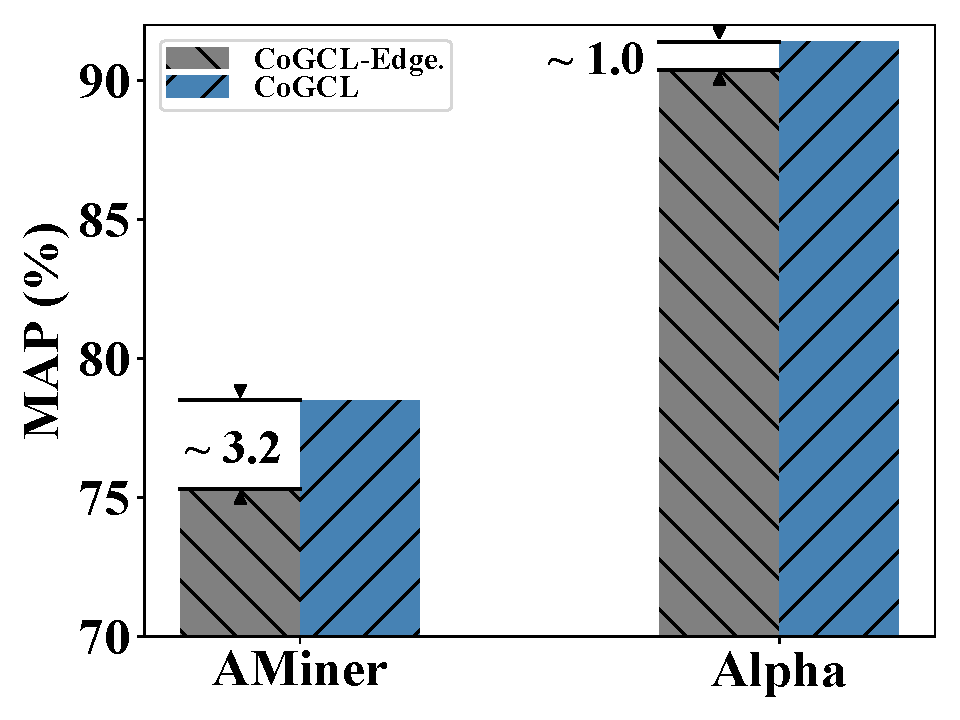
\includegraphics[width=0.2\textwidth]{figures/hardcases}
	}
	\caption{\label{fig:para} The fine-tuning performances under different proportion of the labeled data in four datasets.}
\end{figure*}
}






\subsection{Evaluation of \smodel}


\vpara{Baselines.} We compare \smodel with four general GNNs models, including GCN~\cite{kipf2016semi}, GAT~\cite{velivckovic2017graph}, GraphSAGE~\cite{Graphsage}, and GIN~\cite{xu2018powerful}, and three specific GNN models for anomaly detection, i.e., GeniePath~\cite{liu2019geniepath}, GraphConsis~\cite{liu2020alleviating}, and CARE-GNN~\cite{dou2020enhancing}, which are further introduced in Section~\ref{sec:related}.
%To reduce the negative influence of the suspicious links, GeniePath adopts the LSTM-based attention mechanism, GraphConsis designs neighbor sampling and relation-aware attention strategies, and CARE-GNN applies reinforcement learning to filter noisy neighbors. 
Other GNN-based anomaly detection models such as GAS~\cite{li2019spam}, FdGars~\cite{FdGars}, Semi-GNN~\cite{SemiGNN}, and Player2Vec~\cite{zhang2019key}, are empirically proven to be less powerful than the adopted baselines, thus are ignored in the experiments.
We additionally compare with logistic regression by injecting top eigenvectors as features to perform node classification.  

\hide{
	\begin{itemize}[leftmargin=1em]
	\item \textit{Logistic Regression} Is a non-GCN classifier. Specifically, we feed the eigenvector of a node into logistic regression to predict whether it is an anomaly or not.  	
	\item \textit{GeniePath}~\cite{liu2019geniepath} Is GNN-based method which learns the neighborhood aggregation functions using LSTM and attention mechanism. It assigns low weights to the suspicious links for mitigating their negative influence.
	\item \textit{GraphConsis}~\cite{liu2020alleviating} Proposes three mechanisms of context embedding, neighbor sampling, and relation attention to address the inconsistency problems cased by anomalies.
	\item \textit{CARE-GNN}~\cite{dou2020enhancing} Modifies neighborhood aggregation process of GNNs via deep reinforcement learning. It gets rid of pre-defined thresholds and can be easily incorporated into other GNN-based frameworks. 
\end{itemize}
}



\begin{table}
	\newcolumntype{?}{!{\vrule width 1pt}}
	\newcolumntype{C}{>{\centering\arraybackslash}p{2.5em}}
	\renewcommand\tabcolsep{3.5pt} 
	\caption{
		\label{tb:ablation_study} Ablation Studies of \model (\%). We adopt the best node update strategy, i.e., GCN for Multi-graph datasets and GIN for Single-graph datasets.
	}
	\footnotesize
	\scriptsize
	%\centering 
	\renewcommand\arraystretch{1.0}
	\begin{tabular}{@{~}l?@{~}*{1}{CC?}*{1}{CC?}*{1}{CC?}*{1}{CC}@{~}}
		\toprule
		\multirow{3}{*}{\vspace{-0.3cm} Model}
		&\multicolumn{4}{c?}{\textbf{Multi-graph (GCN)}}
		&\multicolumn{4}{c}{\textbf{Single-graph (GIN)}} 
		
		\\
		\cmidrule{2-5} \cmidrule{6-9}
		&\multicolumn{2}{c?}{\textbf{AMiner}}
		&\multicolumn{2}{c?}{\textbf{MAS}} 
		&\multicolumn{2}{c?}{\textbf{Alpha}} 
		&\multicolumn{2}{c}{\textbf{Yelp}} 
		
		\\
		\cmidrule{2-3} \cmidrule{4-5} \cmidrule{6-7} \cmidrule{8-9}
		& {AUC} & {MAP} & {AUC} & {MAP} & {AUC} & {MAP} & {AUC} & {MAP}   \\
		\midrule
		\textbf{\model}
		&\textbf{89.84}    & \textbf{78.73} &  \textbf{87.62}  & \textbf{75.18} & \textbf{90.53}  & \textbf{91.20}  & \textbf{79.64} &  \textbf{37.15}     \\	
		\midrule
		\multicolumn{9}{c}{\textbf{Variant Loss Functions}} \\
		\midrule
		+ CE\_loss
		&80.30   & 61.02 & 81.53  & 67.42 & 88.64  & 89.10  & 79.18 & 37.05   \\	
		\midrule
		\multicolumn{9}{c}{\textbf{Variant Edge Update Strategies}} \\
		\midrule
		- LP\_constraint
		& 89.36  &78.57 & 87.25  & 74.56  & 89.70  & 90.55  & 78.63 & 35.62   \\
		- Global Info.
		& 88.67 & 77.13 & 86.78  & 73.48  & 89.93  & 90.63  & 78.61 & 35.20   \\	
		- Edge Update
		& 88.21 & 76.97 & 86.34  & 71.54 & 89.69  & 89.86  & 78.51 & 35.19   \\	
		\midrule
		\multicolumn{9}{c}{\textbf{Variant Node Update Strategies}} \\
		\midrule
		$\modelgcn$
		&\textbf{89.84}    & \textbf{78.73} & \textbf{87.62}  & \textbf{75.18} & 85.07  & 87.09  & 73.33 & 30.64   \\	
		$\modelgat$
		& 89.00 & 77.98 & 86.30  & 72.75 & 83.26  & 86.37  & 72.87 & 29.91   \\	
		$\modelsage$
		& 87.84  & 75.26 & 82.86  & 68.52  & 86.54  & 87.07  & 76.52  & 33.28   \\	
		$\modelgin$
		& 89.04   & 77.02 & 83.39  & 67.46 & \textbf{90.53}  & \textbf{91.20}  & \textbf{79.64} &  \textbf{37.15}  \\	
		\midrule
		\multicolumn{9}{c}{\textbf{Variant Graph Update Strategies}} \\
		\midrule	
		+ Avg Pooling
		& 89.01 & 77.66 & 86.39  & 72.73 & 89.02  & 89.57  & 78.70 & 34.55   \\
		+ Sum Pooling
		& 86.95 & 72.09 & 86.45  & 73.98 & 88.01  & 86.69   & 76.79 & 34.11   \\
		+ Max Pooling
		& 80.91 & 61.97 & 84.06  & 70.52 & 89.25  & 88.56  & 78.54 & 33.96   \\
		\bottomrule
	\end{tabular}
	
\end{table}

\vpara{Setup.}
%For AMiner and MAS, we select 70\% researchers' graphs as the training data and use the remaining ones as the test set. During training, we perform the graph convolution on each graph and use all the nodes in it to compute the loss function in Eq.\eqref{eq:loss}. For testing, we first rank nodes based on their cosine similarities calculated between node embeddings with their corresponding graph context embeddings in ascending order,  then we evaluate AUC and MAP for the ranked nodes in each test graph and average the metrics of all the test graphs as the final metrics.For Alpha and Yelp, we select 75\% labeled nodes from the single graph as the training data and use the remaining ones as the test set. We perform the graph convolution on the single graph, use all the nodes in the training set to compute the loss function, and evaluate AUC and MAP for the ranked nodes in the test data.
For the multi-graph datasets, i.e., AMiner and MAS, we extract 70\% graphs as the training set, 10\% as the validation set, and 20\% as the test set. During training, we perform \smodel on each graph following Algorithm~\ref{algo:training}. For testing, we rank nodes based on the cosine similarities between their node embeddings and the corresponding graph context in an ascending order, then we evaluate AUC and MAP of each graph and average the metrics of all test graphs as the final metrics. 
For the single-graph datasets, i.e. Alpha and Yelp, we also extract 70\% of labeled nodes from the single graph as the training data, 10\% as the validation set, and 20\% as the test set. We perform \smodel on the single graph, and evaluate AUC and MAP for the ranked nodes in the test data. Notably, for GraphConsis and CARE-GNN whose inputs are the graph with multi-relation links, we use its multi-relation information, while \smodel merges multi-relation links between two nodes into single-relation links.
% For all experiments, we run 5 trials and report the mean results.
We run 5 trials and report the mean results.


\vpara{Implementation.} 
For \smodel, the number of layers $L$ is empirically set as 2, the temperature hyperparameter $\tau$ is set as 0.1 in Eq.~\eqref{eq:loss}, and $\lambda$ is set as 0.6 in Eq.~\eqref{eq:GUMBEL}. We use Adam with learning rate 1$\times 10^{-3}$ for training. The learning rate is set as the initial value over the first 10\% steps, and then linearly decay to 1/10 of the initial value. 

For the GCN, GAT, GraphSAGE, and GIN, We leverage the implementations provided by Pytorch Geometric\footnote{https://github.com/rusty1s/pytorch\_geometric}, and set the number of convolutional layers as 2 for all general GNNs. For GeniePath, GraphConsis, and CARE-GNN, we use the authors' official codes with the same training settings. The data format is transformed appropriately to fit their settings. All models are running on Python 3.7.3, 1 NVIDIA Tesla V100 GPU, 512GB RAM, Intel(R) Xeon(R) Gold 5120 CPU @ 2.20GHz.


\vpara{Overall Results.} 
Table \ref{tb:overall_res} presents the performance of \smodel and all the comparison methods on four datasets. We can see that,  \smodel substantially improves over all other baselines, +2.5-27.35\% in AUC and +0.31-28.06\% in MAP, on all the datasets. Among all the baselines, logistic regression performs the worst as it only leverages the structural information and does not apply graph convolution to integrate neighbor messages. None of the specific graph-based anomaly detection methods can keep the advantage over the general GNNs on all the datasets. For example, GraphConsis~\cite{liu2020alleviating} performs worse than GIN~\cite{xu2018powerful} on AMiner. 
%which reveals the dedicated structure for anomaly detection can not maintain its strength in different scenarios. 
The highlighted results in the table are from \model, which adopts the context-aware contrastive objective and the  three-stage GNN encoder, performing stably the best over all the datasets.

\begin{figure}[t]
	\centering
	\subfigure[\smodel vs. w/o EdgeU]{\label{subfig:hard_case}
		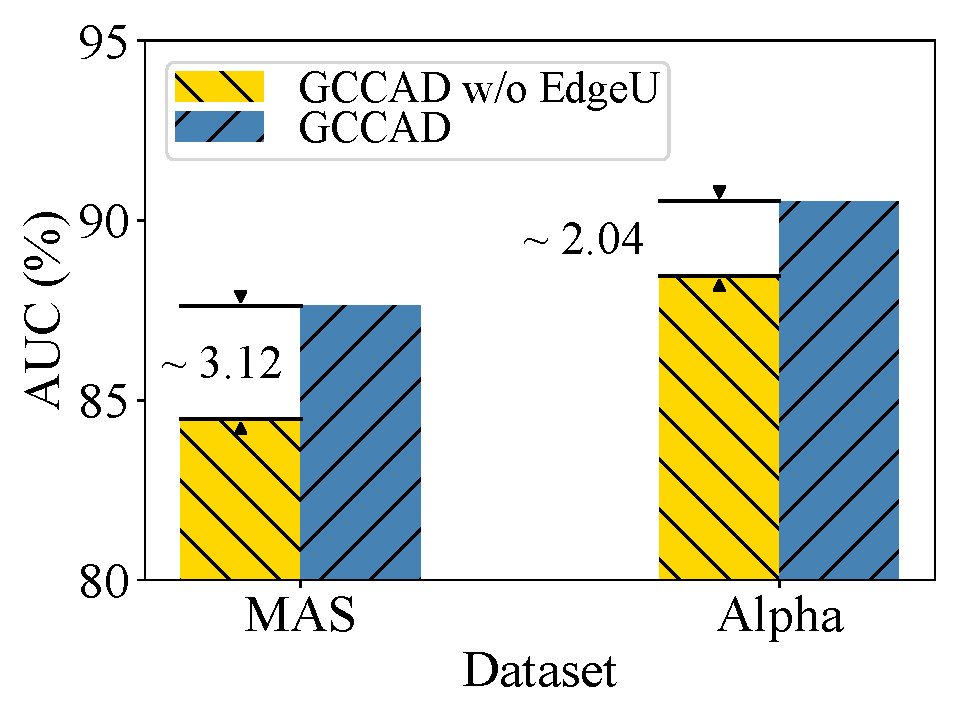
\includegraphics[width=0.23\textwidth]{figures/hard_cases}
	}
	\hspace{-0.1in}
	\subfigure[MAP vs. Corrupt Ratio]{\label{subfig:corrupt_ratio}
		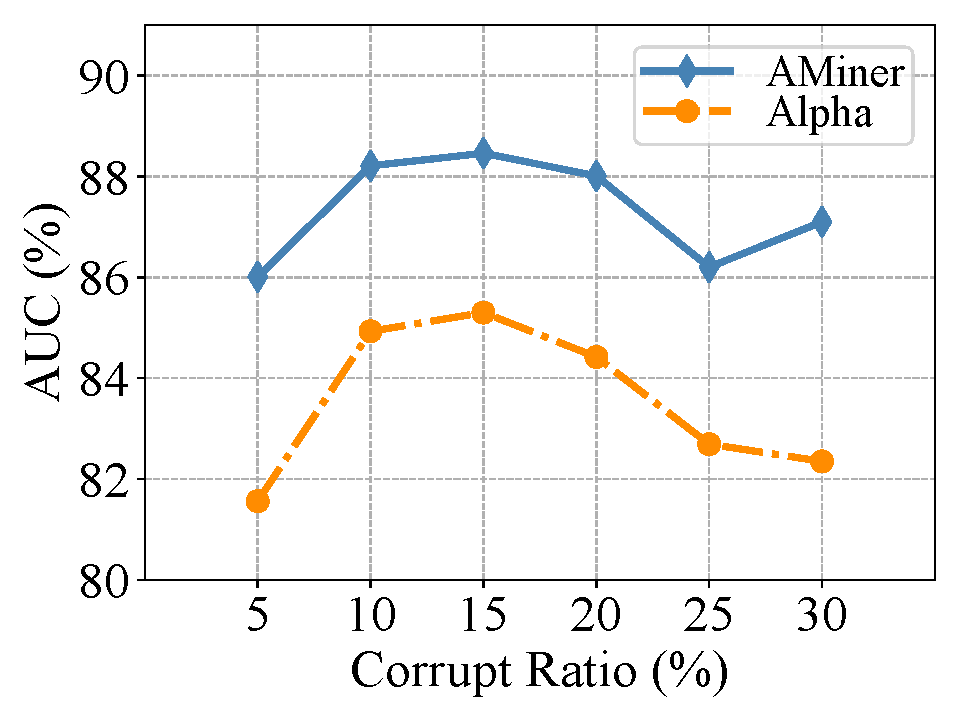
\includegraphics[width=0.23\textwidth]{figures/corrupt_ratio}
	}
	\caption{\label{fig:hyperparameters} We study (a) the performance gain of the supervised \smodel obtained by edge update step on the filtered Alpha and MAS datasets;  (b) the best AUC of \spmodel without fine-tuning when varying the corrupt ratio, i.e., the ratio of the injected abnormal nodes, on AMiner and Alpha.}
\end{figure}





%From Table~\ref{tb:overall_res}, we can also see the performance gain over the best baseline obtained by \smodel on AMiner and MAS (6.59-11.70\% in AUC) is much higher than that on Alpha and Yelp (0.85-1.62\% in AUC). Because as shown in Table~\ref{tb:dataset}, Alpha's concentration, measured by the average cosine similarity of all pairs of nodes, is the largest among all the datasets. The metric indicates Alpha is least diverse, making it easy to distinguish anomalies from others on Alpha. Thus the performance on Alpha is the highest. Such a slightly consistent dataset makes the baselines via binary classification work well and relatively reduces the performance gain of the contrastive learning of \model.In contrast, compared with AMiner and MAS, Yelp is too diverse to discover a unique normal pattern from the entire graph, making \smodel less prominent on Yelp than on AMiner and MAS.




%With respect to different GNNs-variants, they simply propagate node information via neighborhood aggregation without distinguishing the negative influence provided by suspicious links. Graph-based anomaly detection methods further locate and tackle this issues. Among this, Logistic Regression detects anomalies solely based on node's structure role without incorporating neighborhoods information and attribute characteristics, thus it performs worser than GNN-variants. GeniePath learns to mitigate these negative influences by assigning low weights to the suspicious links via attention mechanism. However, the suspicious links are not thoroughly removed. GraphConsis and CARE-GCN additionally tackle these problems via removing suspicious links before graph convolution step in a decoupled way. However, they only use the raw features of nodes to determine the link probability. Most prominently, all above methods formalize anomaly detection problem as a binary node classification scenario. Instead, \smodel analytically and empirically determines a node's label based on its global context. For this, a graph context contrastive loss function and context-aware encoder are proposed to incorporate the information of global context. Thus, \smodel have the superior detecting performance that other baselines. 

  

%Actually, the real feature distributions among normal and abnormal nodes are diverse (see. \secref{sec:intro}), therefore it is hard to find a clear boundary to split normal and abnormal nodes.

%Compared to Logistic Regression 

%thus they perform worser than graph-based anomaly detection methods is 
%In data-view, \smodel outperforms others baselines by 1.01 $\sim$ 10.43\% in AUC among all datasets





\vpara{Ablation Studies.} To this end, there have two major differences: the context-aware contrastive objective and the three-stage GNN encoder between \smodel and other baselines. Thus we conduct the ablation studies to verify the efficacy of different components in \model.  The four main model variants are presented as follows, and the results are illustrated in Table~\ref{tb:ablation_study}. 


\begin{itemize}[leftmargin=1em]
	\item \textbf{w/ CE\_loss:} Change the contrastive loss in Eq.~\eqref{eq:loss} with cross-entropy objective.
    \item \textbf{Edge Update Strategies:} Change the edge update component in \secref{subsec:edge} to \textit{w/o LP\_constraint} that removes the constraint loss $\mathcal{L}_{\text{link}}$ in Eq~\eqref{eq:constraint},  
	\textit{w/o Global Info.} that removes $(\boldsymbol{h}^{(l-1)}_{(i/j)} - \boldsymbol{q}^{(l-1)})$ in Eq.\eqref{eq:linkage_likelihood}, or \textit{w/o Edge Update} that removes the entire edge update step.
	\item \textbf{Node Update Strategies:} Change the node update strategies in Eq.~(\ref{eq:aggregation}) and Eq.~(\ref{eq:combination}) to the node update strategies in GCN, GAT, GraphSAGE, or GIN. 
	\item \textbf{Graph Update Strategies:} Change the memory-based readout function in Eq.\eqref{eq:readout} to average pooling (\textit{Ave Pooling}), sum pooling (\textit{Sum Pooling}), and maximal pooling (\textit{Max Pooling}) of all the nodes.
\end{itemize}

%\ipara{Results. }The results are shown in Table~\ref{tb:ablation_study}. 


\ipara{Node Update Strategies.}  From Table~\ref{tb:ablation_study}, we can see that 
\smodel with various node update strategies outperforms other baselines in most cases, which suggests the superiority of context-aware contrastive objective and the three-stage GNN encoder.

We also observe that different strategies have the performance gap, with less than 6\% in AUC and 7\% in MAP.  On the multi-graph datasets, \smodel performs the best with the mean AGGREGATION and the concatenation COMBINE strategies in GCN~\cite{kipf2016semi}, while on the single-graph datasets, it performs the best with the sum AGGREGATION and the concatenation COMBINE strategies in GIN~\cite{xu2018powerful}. Obviously, the trend of performance changes over different node update strategies is akin to that of general GNNs, as shown at the top of Table~\ref{tb:overall_res}. Thus we conjecture the instability is mainly due to the intrinsic traits of the node update strategy in GNNs. 

Thus, unless stated otherwise, we only conduct experiments of \smodel with the best node update strategy, that is, GCN on the multi-graph datasets and GIN on the single-graph datasets, in the remaining parts.




\ipara{The Contrastive Loss Function.}
From Table~\ref{tb:ablation_study}, we see that the performance gain of \smodel over +CE\_loss on the multi-graph datasets (+6.09-9.54\% in AUC and +7.76-17.71\% in MAP) is much higher than that on the single-graph datasets (+0.46-1.89\% in AUC and +0.60-2.10\% in MAP). 
% Since the multi-graph datasets correspond to the scenario that the data distributions is dynamically changed in different graphs, while the single-graph datasets correspond to the scenario that the data distributions are relatively static,  
Such results empirically validate Theorem 1 that the context-aware contrastive objective is more resilient than cross-entropy in terms of the generation capacity. 
Since the abnormal node distributions in different graphs are usually quite different, the multi-graph setting presents much more diverse abnormal distributions than the single-graph setting. Thus optimizing the entropy of abnormal nodes take a critical role to learn a more generalized model across various graphs. 
What's more, our proposed context-aware contrastive loss performs slightly better than CE\_loss in the single-graph datasets, which shows that our method can tackle the class imbalance issue to some degree.

%, thus the performance gap between \smodel and other baselines on the multi-graph datasets is larger than that on the single-graph datasets. 

%To this end, there have two major differences: the context-aware contrastive objective and the three-stage GNN encoder between \smodel and other baselines. Thus to alleviate the effects caused by GNN encoder of \model, we keep the GNN encoder the same as the proposed three-stage encoder, but change the loss function to the cross-entropy loss, and show the results of +CE\_loss on Table~\ref{tb:ablation_study}. Compared with +CE\_loss, \smodel still achieves 6.09-9.54\% AUC improvements on the multi-graph datasets, while 0.46-1.89\% AUC improvements on the single-graph datasets,  which indicates that the proposed context-aware contrastive loss function makes an significant contribution. 

% when comparing \smodel with baselines, the ablation studies (\smodel vs. \smodel w/ CE\_loss) have already confirmed the contrastive objective mainly contributes to the improvements. 


% \ipara{Objective Functions.} Overall, \smodel outperforms \smodel w/ CE\_loss by up to 9.54\% in AUC and 17.71\% in MAP. However, the performance gain on the multi-graph datasets (6.09-9.54\% in AUC) are larger than that on the single-graph datasets (0.46-0.89\% in AUC), which agrees with the statements from Theorem 1 that the context-aware contrastive loss function is more robust than the cross-entropy loss function to address various scenarios. 


\ipara{Context-aware GNN Encoder.} 
\smodel w/ CE\_loss outperforms other state-of-the-art baselines by up to 17.81\% AUC, which elucidates the powerful representation capability of the proposed context-aware GNN encoder. The improvements can give credit to two perspectives: the context-aware edge update and the memory-based global update. Thus, We further verify the effectiveness of each component.   

\vpara{\ipara{Edge Update Strategies.}} \smodel w/o LP\_constraint performs slightly worse than \model, denoting link prediction loss can not only accelerate the optimization of link predictor but also contribute to the overall improvement. 

\smodel w/o Global Info. underperforms \model, revealing the context-aware link predictor that incorporates the distance to the global context as the implicit supervision, can benefit the suspicious link prediction.

Compared with above two variants, \smodel w/o Edge Update performs the worst (-0.84-1.63\% in AUC), verifying the efficacy of the proposed edge update mechanism. However, the performance enhancement brought by the edge update is not significant. We speculate the norm links which connect the nodes of the same labels occupy the majority of all the links (e.g., 90.5\% on AMiner and 84.4\% on MAS in Table.~\ref{tb:dataset}). Thus, removing the small amount of suspicious links by the link predictor can only exert limited effect. To verify this, we select the hard instances, i.e., the abnormal nodes that connect at least $k$\footnote{Empirically, $k$ is set as 1 in MAS and 3 in Alpha respectively.} normal nodes, from both MAS and Alpha, and re-evaluate the variants on filtered datasets. From Fig.~\ref{subfig:hard_case}, we can see that \smodel significantly outperforms w/o Edge Update by 3.12\% and 2.04\% AUC on the two datasets, respectively. The results indicate that the negative influence of the suspicious links can be effectively reduced by the edge update step.   

\vpara{\ipara{Global Update Strategies.}} The proposed memory-based global context update mechanism performs the best, which improves 0.83-8.93\% AUC and 1.07-16.76\% MAP over other variant mechanisms. Because the memory that records the global context of the last layer can help estimate the contribution of each node in the current layer, thus it will benefit the generation of precise global context in the current layer.

%underperforms \smodel (reduces 0.45-1.16\% in AUC), which indicates the context-aware link predictor injecting the relative distance to the global context as the feature can benefit the suspicious link prediction. \smodel w/o EdgeU is comparable to \smodel on AMiner, MAS and Yelp, and even performs slightly better than it on Alpha.
%To figure out this, we further count the ratio between benign and suspicious edges among different datasets. Results show that the number of benign edges take over 80\% of whole edges on all datasets\footnote{We do not count this ratio on Alpha, because its ground truth is partially labeled.}. Based on the observation, we conjecture that benign edges are dominant in the graph convolution step. Even a few propagation of suspicious edges are pruned during Edge Update, it still can not generate a huge impact on overall performance. 
%As normal links, that connects the nodes of the same labels, occupy the majority of all the links on AMiner, MAS, and Yelp\footnote{Alpha is partially labeled and cannot state the normal link ratio.}, we conjecture that the normal links dominate the performance of the graph convolution, making the small amount of the suspicious links impact less on the graph convolution process.
%To further verify the conjectures and effectiveness of the edge update step, we select the hard instances, the abnormal nodes that connect at least $k$\footnote{Empirically, k is set as 1 in MAS, and 3 in Alpha respectively.} normal nodes, from both MAS and Alpha, and re-evaluate \smodel and the variant w/o EdgeU on the filtered datasets. From Figure~\ref{subfig:hard_case}, we can see that \smodel significantly outperforms w/o-EdgeU by 3.12\% and 2.04\% AUC on the two datasets respectively. The results imply that the negative influence of the suspicious links can be effectively reduced by the edge update step.   




\begin{table}
	\newcolumntype{?}{!{\vrule width 1pt}}
	\newcolumntype{C}{>{\centering\arraybackslash}p{6em}}
	\renewcommand\tabcolsep{2.5pt} 
	\caption{
		\label{tb:tansferLearning} Transfer Learning about Cross-Entropy (CE) and Context Contrastive Loss (CL) on AMiner and MAS (AUC \%). The model trained on one dataset (top) and evaluate on another one (left).
	}
	\footnotesize
	\scriptsize
	\centering 
	\renewcommand\arraystretch{1.0}
	\begin{tabular}{@{~}l@{~}*{1}{?C?CC?CC}@{~}}
		\toprule
		\multicolumn{2}{c?}{Model} &\textbf{AMiner} & \textbf{MAS} & \textbf{Performance Drop}\\
		\midrule
		\multirow{2}{*}{\textbf{AMiner}}& w/ CL & 89.84 & 87.70 & \textbf{2.14}\\ 
		%\cmidrule{2-5}
		&w/ CE & 80.30 &77.05  & 3.25 \\
		\midrule
		\multirow{2}{*}{\textbf{MAS}}& w/ CL & 84.41  &  87.62 & \textbf{3.21}\\ 
		%\cmidrule{2-5}
		&w/ CE & 74.15 & 81.53 & 7.38 \\
		\bottomrule
	\end{tabular}
	
\end{table}

\hide{
\begin{table}
	\newcolumntype{?}{!{\vrule width 1pt}}
	\newcolumntype{C}{>{\centering\arraybackslash}p{6em}}
	\renewcommand\tabcolsep{2.5pt} 
	\caption{
	\label{tb:tansferLearning} Transfer Learning about Cross-Entropy (CE) and Context Contrastive Loss (CL) on AMiner and MAS (AUC \%). The model trained on one dataset and evaluate on another one.
}
	\footnotesize
	\scriptsize
	\centering 
	\renewcommand\arraystretch{1.0}
	\begin{tabular}{@{~}l@{~}*{1}{?C?CC?CC}@{~}}
		\toprule
		\multicolumn{2}{c?}{Model} &\textbf{AMiner} & \textbf{MAS} & \textbf{Performance Drop}\\
		\midrule
    	\multirow{2}{*}{\textbf{AMiner}}& w/ CL &72.10 &68.16 & 3.94\\ 
    	%\cmidrule{2-5}
		&w/ CE &70.23 &57.58 & \textbf{12.65} \\
		\midrule
    	\multirow{2}{*}{\textbf{MAS}}& w/ CL & 74.63 & 72.53 & 2.10 \\ 
    	%\cmidrule{2-5}
		&w/ CE & 72.49 & 66.16 & \textbf{6.33} \\
		\bottomrule
	\end{tabular}
	
\end{table}
}

\vpara{Transfer Learning.} To further investigate the robustness of context-aware contrastive loss compared with cross-entropy objective, we train \smodel and its variant w/ CE\_loss on AMiner/MAS and evaluate them on MAS/AMiner\footnote{Since the feature initialization process and the embedding dimension of Alpha and Yelp are obviously different from each other, we only conduct the transfer learning experiments between AMiner and MAS.}. As shown in Table~\ref{tb:tansferLearning}, the performance drop of \smodel (-2.14-3.21\% in AUC) is substantially less than that of  w/ CE\_loss (3.25-7.38\% in AUC) under the setting of transfer learning, which shows the superior robustness ability of the context-aware contrastive objective compared with the cross-entropy objective. 





% \vpara{Case Study.} We visualize the author ``Jun Lu", a professor from Yale University, from Google Scholar's published author profile data as a case study. As the news\footnote{https://www.universityworldnews.com/post.php?story=\\20120807160325397} 
% reported in 2012 that another researcher named ``Jun Lu" from Beijing University of Chemical Technology cheated the awards using the papers of ``Jun Lu" from Yale. This event caused by the wrongly assigned papers of the same author name implies the importance of anomaly detection. We show the changes of similarities between right and wrong-assigned papers to the global context before and after adopting \model, as illustrate in \figref{fig:case}. \smodel effectively discriminates the wrongly assigned papers from the right ones by their relative distance to the global context.  




%Table \ref{tb:overall_res} shows the performances of different model variants on four datasets. \model-Context determines the link probability of each node pair solely based on their raw features without incorporating global context information, which can not handle the issues, like two normal nodes which have slightly different features may be misjudged based on their raw features,  result from the diverse node feature distribution. Thus it performs worser that \smodel by up to 1.14\% in AUC and 1.47\% in MAP. Compared with \model, \model+Attention\footnote{As we apply GIN as the backbone of Node Update on both Alpha and YelpChi datasets, there are no edge weights during graph convolution step.} views link prediction probability as the attention weights to each edge, thereby it can not thoroughly eliminate the negative influence cased by suspicious links. \model-Edge Update even directly delete the process of mitigating these negative influence. However, experimental results demonstrate that they have  comparable performance with \smodel on four datasets. To figure out this, we further count the ratio between benign and suspicious edges among different datasets. Results show that the number of benign edges take over 80\% of whole edges on all datasets\footnote{We do not count this ratio on Alpha, because its ground truth is partially labeled.}. Based on the observation, we conjecture that benign edges are dominant in the graph convolution step. Even a few propagation of suspicious edges are pruned during Edge Update, it still can not generate a huge impact on overall performance. This phenomenon also explains that GNN-variants without any strategies to mitigate the negative influence still perform on a par with the anomaly detection baselines. To further verify the effectiveness of link predicator, we select the abnormal nodes with at least $k$ edges connected with normal nodes as hard cases on both MAS and Alpha datasets, and test performances between \model and \model-Edge Update. From table~\ref{tb:hard_cases}, we can see that \smodel significantly outperforms \model-Edge Update by up to 5.17\% in MAP on hard cases, which confirms the negative effects cased by suspicious links are effectively removed during Edge Update.   






\subsection{Evaluation of \pmodel}
\label{subsec:pretrain}

\vpara{Baselines.}
We compare \spmodel with the state-of-the-art graph pre-training models, including GAE~\cite{kipf2016variational}, GPT-GNN~\cite{hu2020gpt}, GraphCL~\cite{you2020graph}, and the graph pre-training models tailored for anomaly detection, DCI~\cite{wang2021decoupling}, ANEMONE~\cite{jin2021anemone}, CoLA~\cite{liu2021anomaly}, in the unsupervised setting. 
GAE is to preserve the structural correlations via reconstructing the vertex adjacency matrix. In addition to the structural correlations, GPT-GNN preserves the attribute interplays via predicting the masked attributes. 
GraphCL maximizes the mutual information of two instances of the same graph obtained by graph data augmentation.  
DCI~\cite{wang2021decoupling} is a cluster-based version of DGI, 
which maximizes the fine-grained mutual information between the embeddings of a cluster and the nodes within it and is proved to be effective for graph anomaly detection. 
ANEMONE and CoLA both underperform the proposed \pmodel. Although ANEMONE and CoLA propose a similar node to sub-graph contrast learning, they sample the sub-graphs by the local random walking algorithm instead of the global clustering algorithm in \pmodel. The latter can result in more diverse normal samples that are more difficult to be distinguished. On the contrary, the former ignores such difficult normal samples during training, which will reduce the model generalization.
For a fair comparison, all the pre-training models adopt the same GNN encoder as \model.



% \begin{figure}[t]
% 	\centering
% 	%\hspace{-0.2in}
% 	%\subfigure[AMiner]{\label{subfig:paper_network}
% 	%	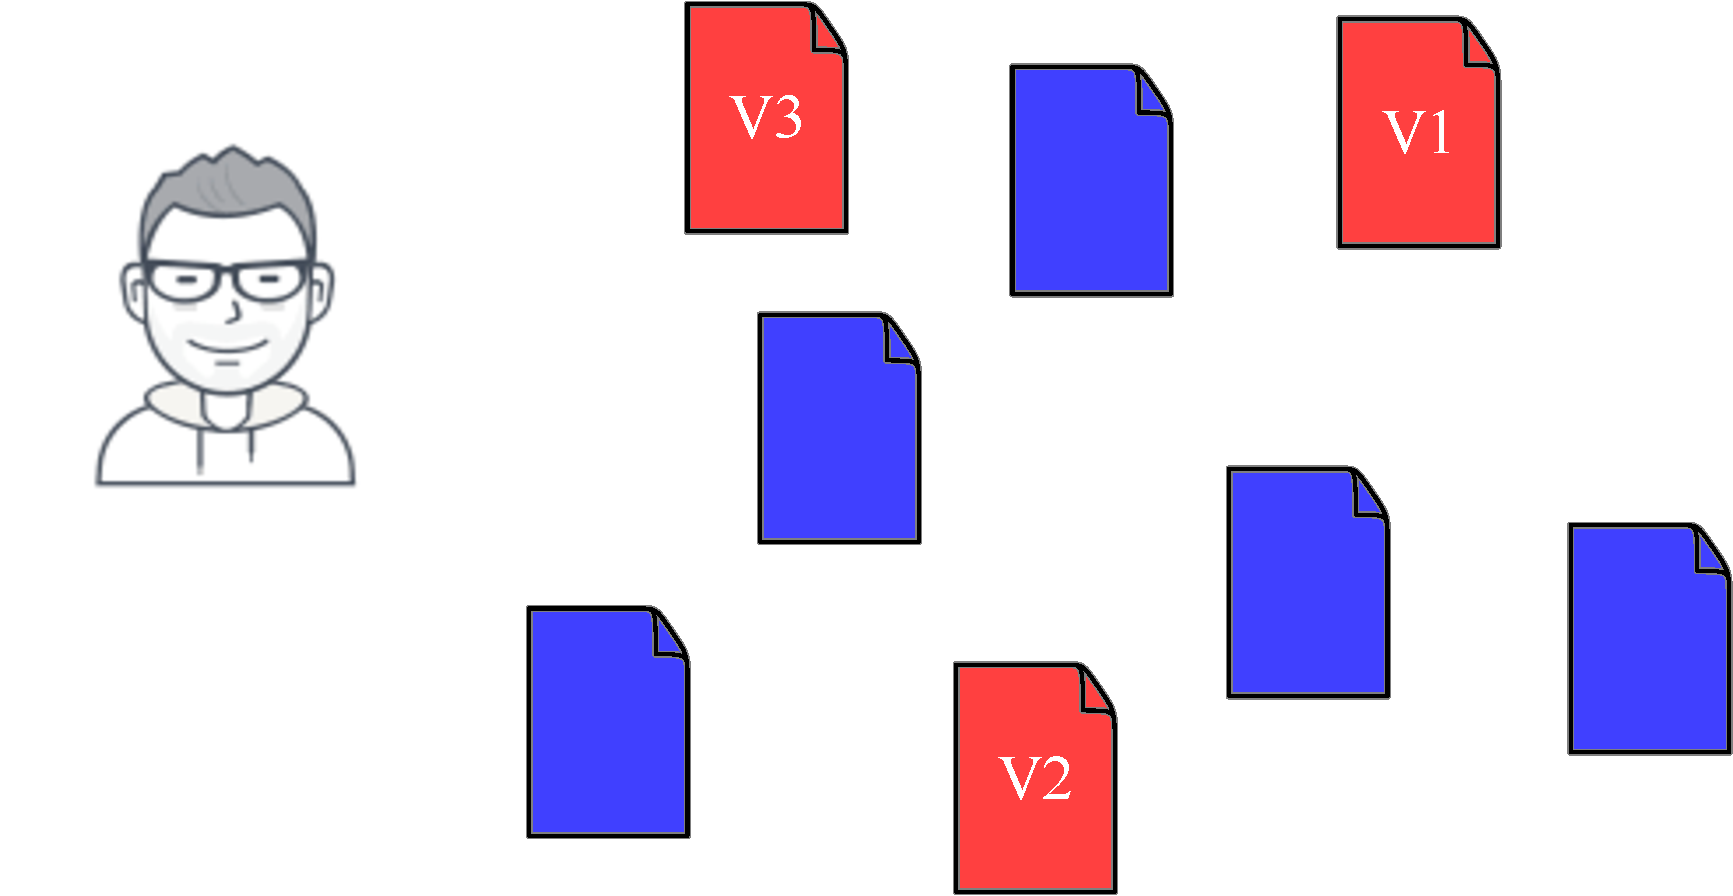
\includegraphics[width=0.33\textwidth]{figures/motivation}
% 	%}
% 	\subfigure[Before]{\label{subfig:t-sne}
% 		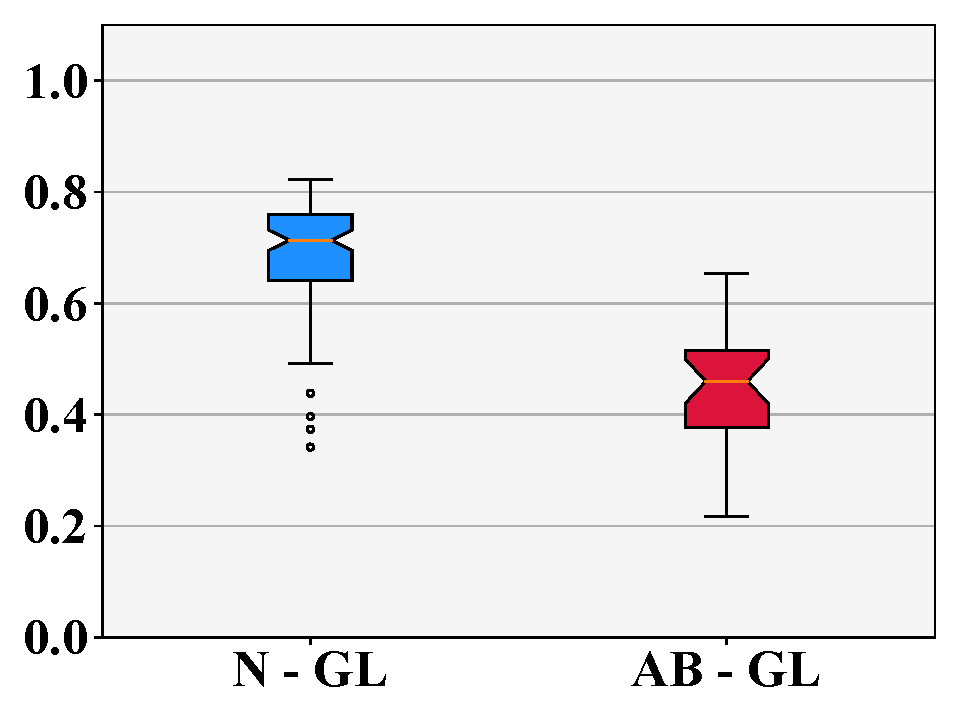
\includegraphics[width=0.23\textwidth]{figures/caseBefore}
% 	}
% 	%\hspace{-0.1in}
% 	\subfigure[After]{\label{subfig:gcn_sim}
% 		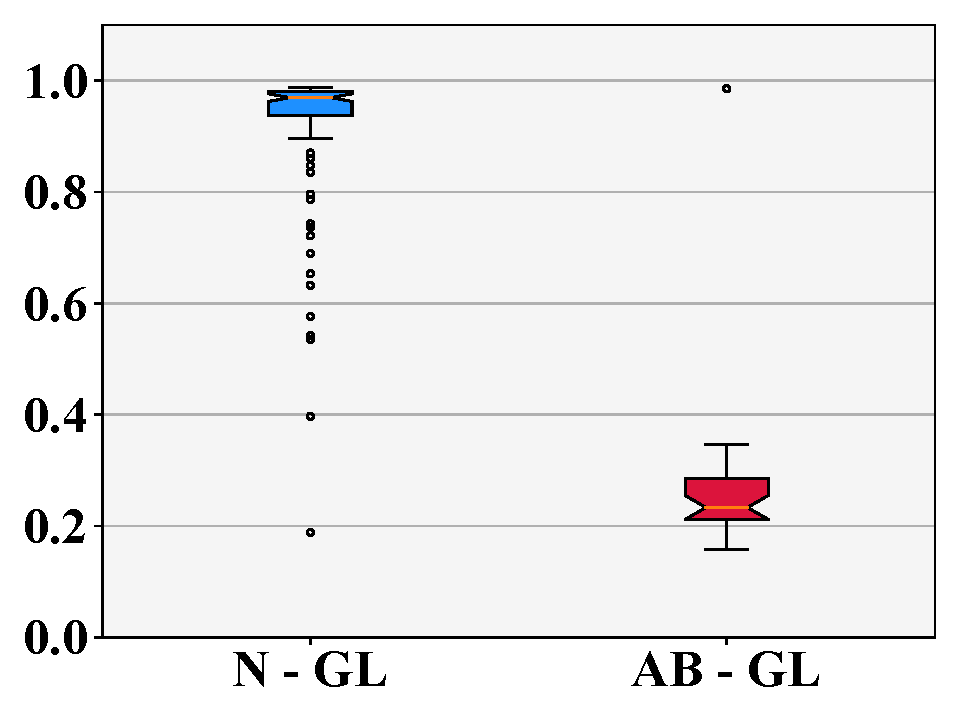
\includegraphics[width=0.23\textwidth]{figures/caseAfter}
% 	}
% 	\caption{\label{fig:case} A real example of detecting the papers that don't belong to ``Jun Lu". %, a professor from University of Munich. 
% 		The similarities between right papers and the global context (blue) vs. that between wrongly-assigned papers and the global context (red) by using input features (a) or embeddings yielded by \smodel(b).} 
% \end{figure}

\vpara{Datasets.} 
In the online AMiner system, we hide the labeled 1,104 graphs in Table~\ref{tb:dataset} and extract additional 4,800 corrupt graphs from it. According to the multi-graph corrupting strategy in~\secref{subsec:self}, we first build a single large paper graph for the whole extracted AMiner dataset and then divide it into multiple graphs according to the ownership of papers to different researchers. For each graph, we corrupt it by injecting the papers from other researchers' graphs as the anomalies with a certain corrupt ratio of 15\%, i.e., the ratio between the number of injected nodes with the number of existing nodes in the graph. The links in the original graph are kept between the nodes in corrupt graphs. Then we build the MAS corrupting graph dataset in the same way.

For the single-graph datasets, Alpha and Yelp, we first cluster it into $K$ sub-graphs by classic K-means algorithm based on their input features. 
We perform the clustering algorithm based on the feature information instead of the structure information, because structural information is more preferred to be tampered than the feature information by the abnormal users. Although the abnormal users might perform both the attribute abnormal behaviors which result in the corrupted features and the abnormal structural behaviors which result in the suspicious links between users, the latter can produce a more negative impact on the whole graph. For example, in social network, a rumor monger usually disguises themselves as regular users by building connections with regular users and dispersing the disinformation via the connections. Thus, identifying suspicious linkages between normal and abnormal ones is more crucial in graph anomaly detection. In light of this, it is inappropriate to split the graphs by the structure information that is highly probably polluted by the suspicious links. We didn’t try to split the graph of Alpha by the feature information, as it is unavailable in the dataset.

The within-cluster correlation is measured by sum-of-squares criterion, namely inertia\footnote{https://scikit-learn.org/stable/modules/clustering.html\#k-means}, estimated by $\sum_{i=0}^{|V|}\min\limits_{\boldsymbol{u}_k\in C}\left(||\boldsymbol{x}_i - \boldsymbol{u}_k||^2\right)$, where $\boldsymbol{u}_k$ is the embeddings of $k$-th cluster center and $C$ is $K$ disjoint clusters. To automatically set a proper $K$, we leverage the Elbow Methods to choose the elbow point of inertia, i.e, to locate the optimal $K^*$ at which the trend of inertia changes from steep to stable (Cf. Fig.~\ref{fig:cluster}). Finally, the graph size $K$ is set as 20 on Alpha and 30 on Yelp.  

%In the online AMiner system, we hide the labeled 1,104 graphs in Table~\ref{tb:dataset} and extract additional 4,800 corrupt graphs from it.  According to Definition~\ref{eq:corrupt} in~\secref{subsec:self}, we first build a single paper graph for the whole AMiner dataset and then divide it  into multiple graphs according to the ownership of papers to different researchers. For each graph, we corrupt it by injecting the papers from other researchers' graphs as the anomalies with a certain corrupt ratio , i.e., the ratio between the number of injected nodes with the number of existing nodes in the graph. The links in the original graph are kept between the nodes in the corrupt graph. We corrupt the MAS graphs in the same way.

%Alpha or Yelp is a single graph itself. We partition it into $K$ graphs by HAC based on the features of the top eigenvectors and corrupt each graph in the same way as corrupting the academic graphs. The graph size $K$, determined by the optimal Silhouette Coefficient, is set as 5 on Alpha and 38 on Yelp,  

\vpara{Setup.} 
%For efficient training on the 4,800 corrupt academic graphs, we include 8 graphs in each batch and sample 48 abnormal nodes and XX normal nodes in each graph. To meet negative instances as much as possible, similar to simCLR~\cite{chen2020simple}, a popular pre-training scheme for visual representation learning, we also include all the nodes from other graphs in the same batch as the negative instances in addition to the pre-injected abnormal nodes in the concerned graph. But different from the pre-injected abnormal nodes, the sampled negative instances from other graphs during training only impact the loss function but are regardless of the graph convolution of the concerned graph. Since the number of the partitioned graphs in Alpha and Yelp is much smaller than that in AMiner and MAS, we set batch size as 1 on them. 
Without any labeled data (0\% labeled data), we train \spmodel and the baselines on the corrupt graphs and evaluate them on the same test set as the supervised \model. Then we also explore the few-shot learning settings, i.e., we further fine-tune the pre-trained models when given a proportion of labeled data.



\begin{figure*}[t]
	\centering
	\subfigure[AMiner]{\label{subfig:aminer}
		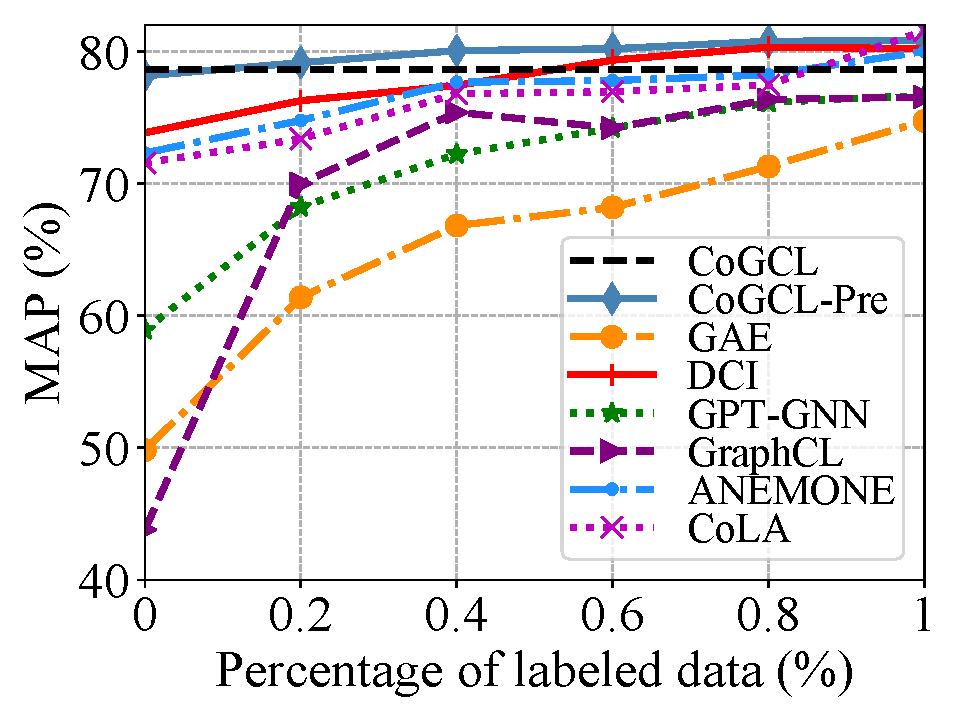
\includegraphics[width=0.24\textwidth]{figures/pretrain_aminer}
	}
	\hspace{-0.1in}
	\subfigure[MAS]{\label{subfig:mas}
		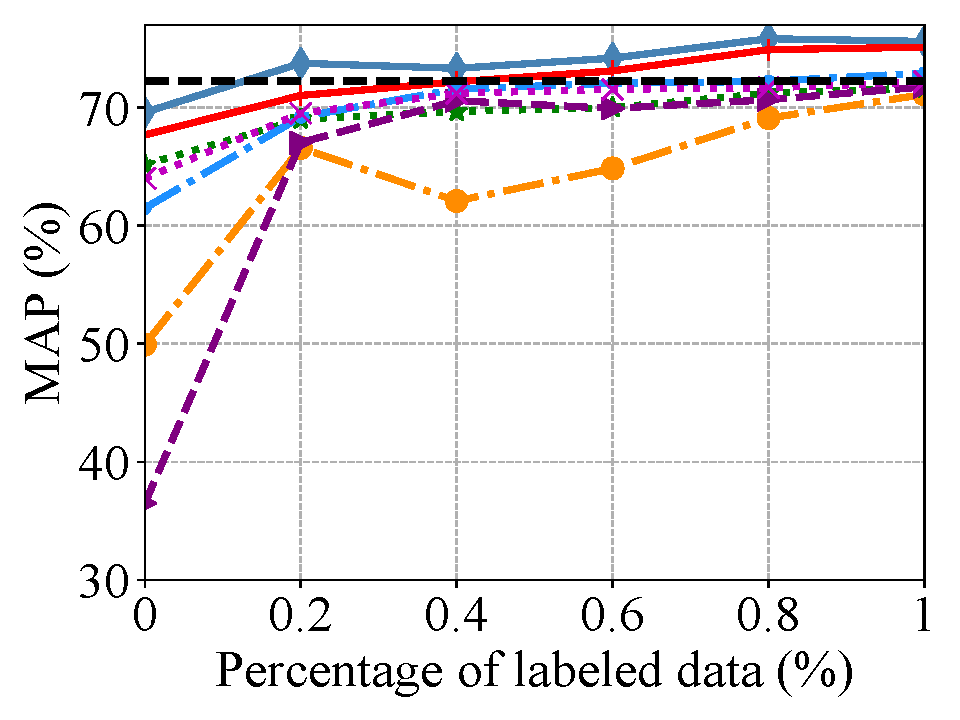
\includegraphics[width=0.24\textwidth]{figures/pretrain_mag}
	}	
	\hspace{-0.1in}
	\subfigure[Alpha]{\label{subfig:alpha}
		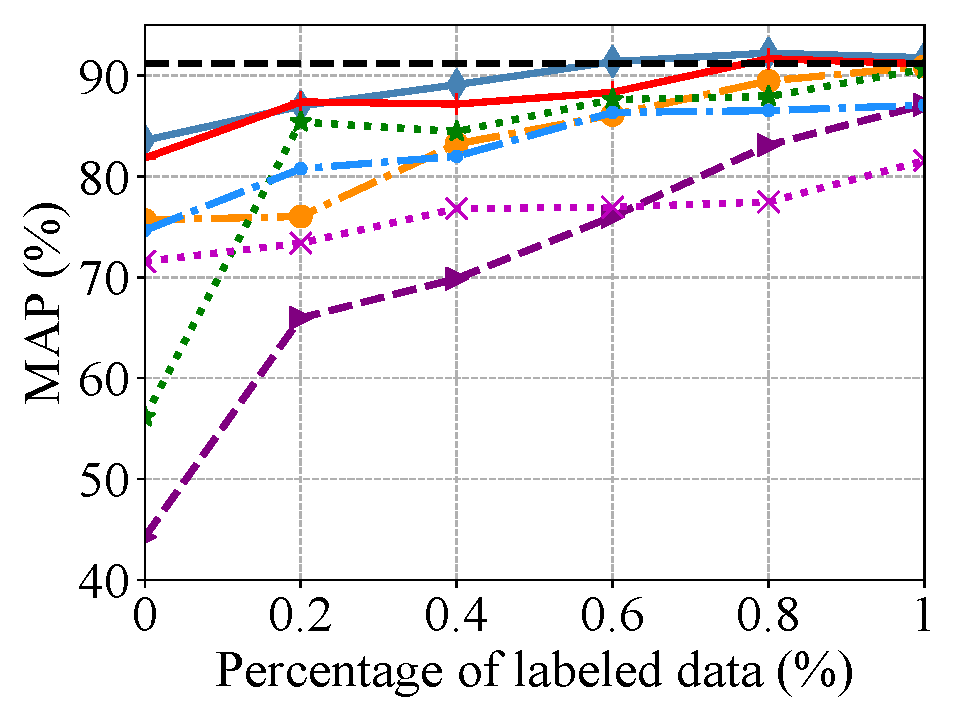
\includegraphics[width=0.24\textwidth]{figures/pretrain_alpha}
	}
	\hspace{-0.1in}
	\subfigure[Yelp]{\label{subfig:yelp}
		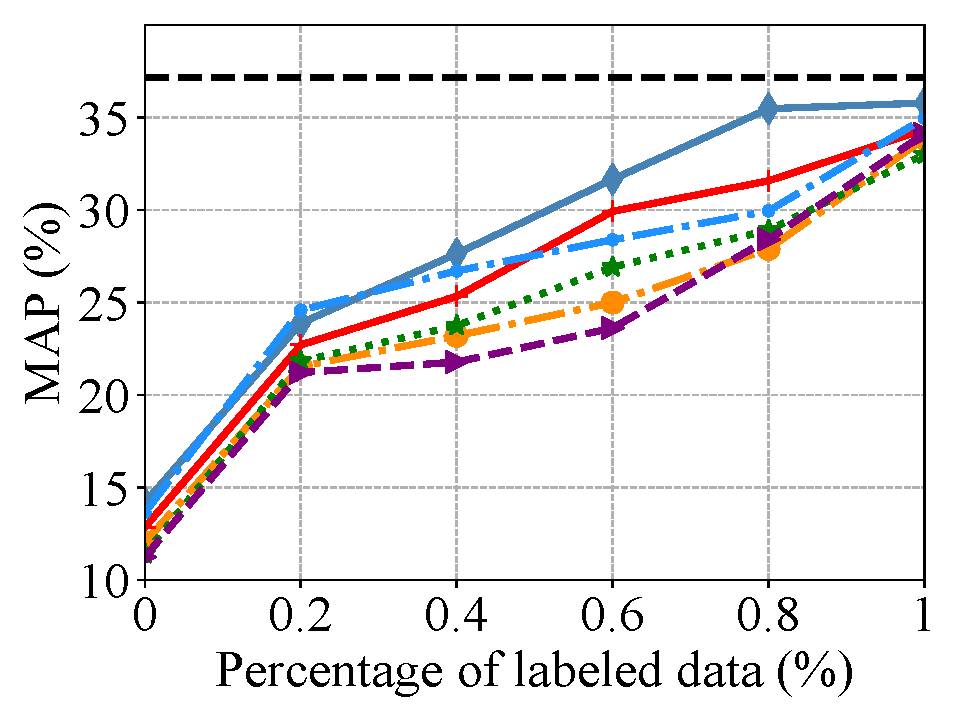
\includegraphics[width=0.24\textwidth]{figures/pretrain_yelp}
	}
	\caption{\label{fig:pretrain} The pre-training and fine-tuning performance given different percentage of the labeled data on four datasets. The horizontal black dashed line represents the performance of the supervised \model.}
\end{figure*}


\vpara{Implementation.} 
For \pmodel, we follow the same setting as \model. For GAE, DCI, GPT-GNN, and GraphCL, we use the authors' official codes with the same training settings. Note that, for GraphCL, we try all the graph augmentation methods defined in the paper and and select the sub-graph augmentation that achieves the best performance in the test set without fine-tuning.

\vpara{Overall Results.} Fig.~\ref{fig:pretrain} shows the pre-training and fine-tuning performance of all the comparison methods given different percentage of labeled data on four datasets. 
From the results, we see that \spmodel (blue line) fine-tuned on 0\%, 10\%, and 60\% labeled data is comparable with the fully-supervised \smodel (black dashed line) on AMiner, MAS, and Alpha respectively. 
What's more, when \spmodel is fined-tuned on all the labeled data, it even outperforms \smodel by 1.72\%, 2.19\%, and 1.04\% in AUC on AMiner, MAS, and Alpha respectively, which reveals the effectiveness of the proposed pre-training framework. 

Our model also outperforms all the baselines when whatever percentage of labeled data is provided. 
GAE and GPT-GNN focus on reconstructing the links in the graphs.
GraphCL aims to capture the normal distribution of the whole graphs.
The objective of them is a little far away from anomaly detection. 
DCI performs the best among all the baselines. Given the global context as the query, DCI aims to contrast between the nodes within the sub-graph (normal nodes) and those from other sub-graphs (abnormal nodes). The objective is similar to \pmodel, but different from the corrupted graphs by \pmodel, the anomalies in DCI are thoroughly disconnected from the normal nodes and are independently embedded in other graphs, 
which may reduce the learning difficulty of the pseudo labels compared with the ground-truth labels. 
Both ANEMONE and CoLA under-perform the proposed GCCAD-pre. Although ANEMONE and CoLA propose a similar node to sub-graph contrast learning, they sample the sub-graphs by the local random walking algorithm instead of the global clustering algorithm in GCCAD-pre. The latter can result in more diverse normal samples which are more difficult to be distinguished. On the contrary, the former ignores such difficult normal samples during training, which will reduce the model generalization.

We also observe that on Yelp, none of pre-training models achieve prominent performance without any labeled data. 
On one hand, as shown in Table~\ref{tb:dataset}, because of the smallest concentration, Yelp is the most diverse dataset, which prevents \pmodel, DCI, and GraphCL from discovering the proper normal pattern.
On the other hand, since the ratio of the suspicious links on Yelp, 22.70\%, is the largest among the datasets, GAE and GPT-GNN that target at preserving the link homophily will wrongly reconstruct those noisy links. 
% \textcolor{blue}{The noisy structure information also prevents \spmodel to split sub-graphs rationally.} 
However, \spmodel still performs best compared with other pre-training models on the most of the percentage of labeled data is provided, which implies the ability of \spmodel to distinguish the normal nodes from the abnormal ones.     

\vpara{Corrupt Ratio.}
Fig.~\ref{subfig:corrupt_ratio} presents the correlation between the ratio of the injected nodes (corrupt ratio) and the performance of \spmodel on AMiner and Alpha without fine-tuning. The results show that the best performance is achieved when about 15\% of abnormal nodes are injected. The corrupt ratio is set in the same way as other datasets. 


\vpara{Clustering Number.}
Fig.~\ref{fig:cluster} presents the correlation between the graph (cluster) number $K$ and the inertia gap $\sigma\left(K\right)$ between $K$ and $K+1$ on Alpha and Yelp. The optimal $K^*$ that achieves the best performance of \spmodel without fine-tuning are marked as red. We observe that \spmodel performs the best when $K^*$ (red) is approximately around the elbow point where the trend of inertia changes from steep to stable. Although we choose the elbow points on Yelp, Yelp is so diverse that none of  the graph pre-training methods can achieve desired performance.

\vpara{Features for Clustering.}
We compare the effect of the clustering algorithm by the structure information or feature information on the pre-training performance. We perform K-means on the graph of Yelp by the structure information, and the result is much poorer than clustering by the feature information (i.e., 12.56\% versus. 14.17\% in terms of MAP), which indicates the more noisy structural information hampers the clustering as well as the pre-training performance. 


% Figure~\ref{fig:cluster} presents the correlation between the elbow point, where the trend of inertia changes from steep to stable, with respect to the graph (cluster) number $K$ and the performance of \spmodel on Alpha and Yelp, where the x-axis is the cluster number $K$, and the y-axis denotes $\sigma\left(K\right)$ representing the inertia gap between $K$ and $K+1$. We observe that \spmodel performs the best when $K^*$ (red) is around the elbow point. However, although we choose the elbow points on yelp, the best performance of \spmodel is also unsatisfied, because Yelp is so diverse that \spmodel cannot achieve desired performance.

%We present the correlation between the graph (cluster) number $K$ and the best performance of \spmodel on Alpha and Yelp without fine-tuning in Figure~\ref{subfig:k} and Figure~\ref{subfig:auc_k}. The results show that when $K$ equals 5, \spmodel performs the best and the Silhouette Coefficient is also optimal. A clear correlation between $K$ and the best performance is not easy to be found on Yelp, because Yelp is so diverse that \spmodel cannot achieve expected performance whatever $K$ is given.
\begin{figure}[t]
	\centering
	%\hspace{-0.2in}
	%\subfigure[AMiner]{\label{subfig:paper_network}
	%	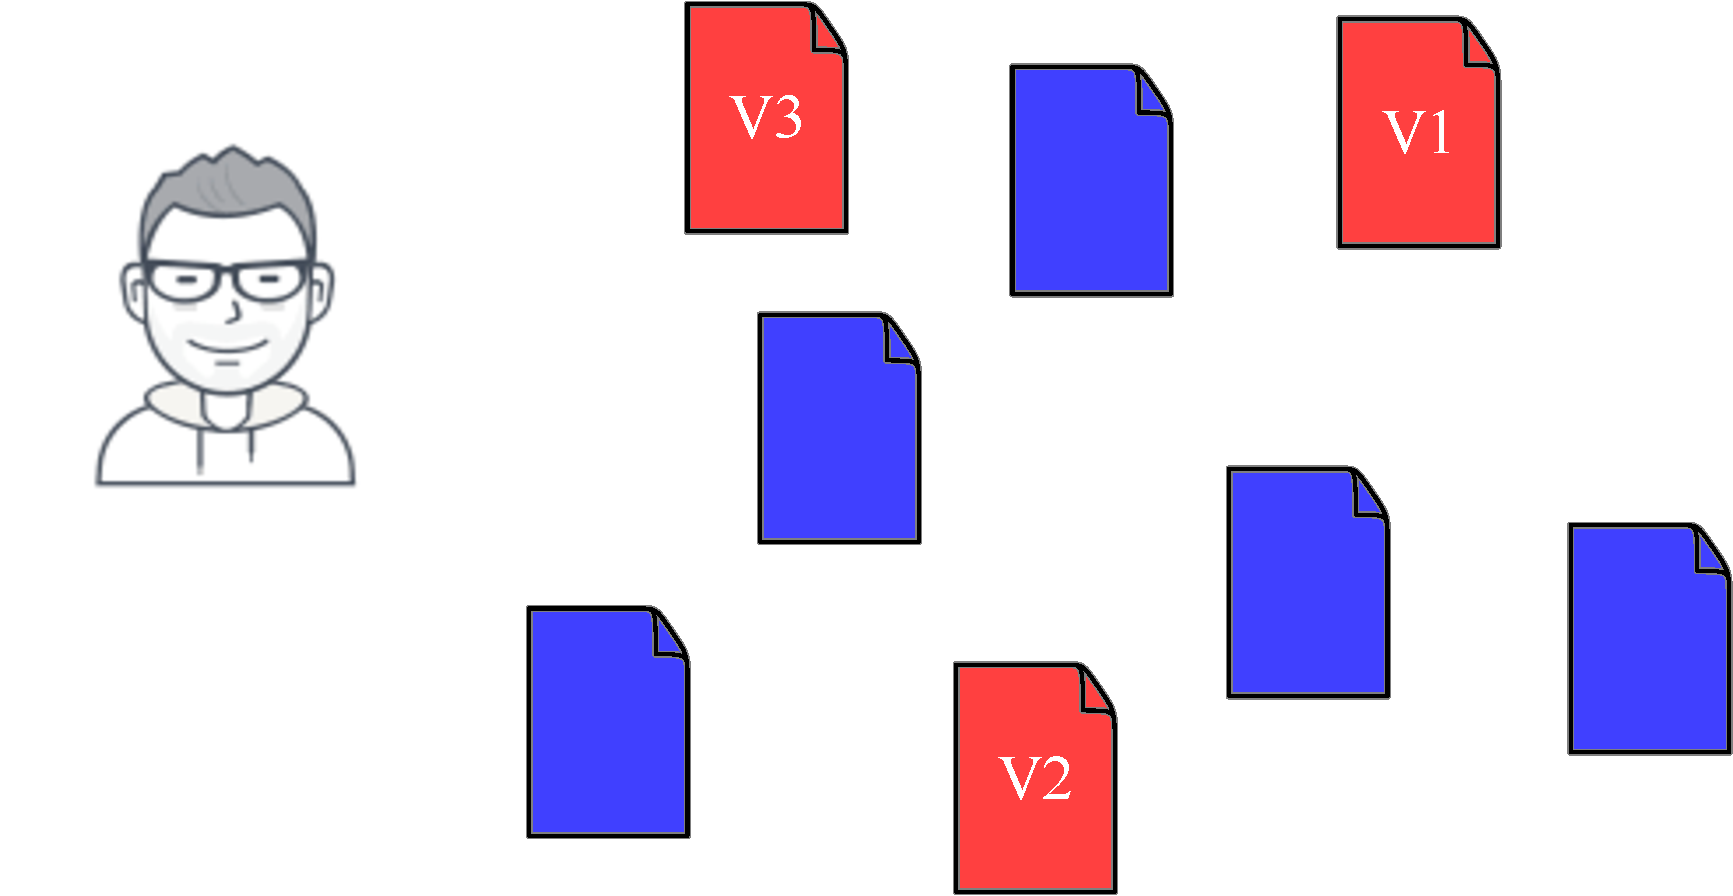
\includegraphics[width=0.33\textwidth]{figures/motivation}
	%}
	\subfigure[Alpha]{\label{subfig:alphaK}
		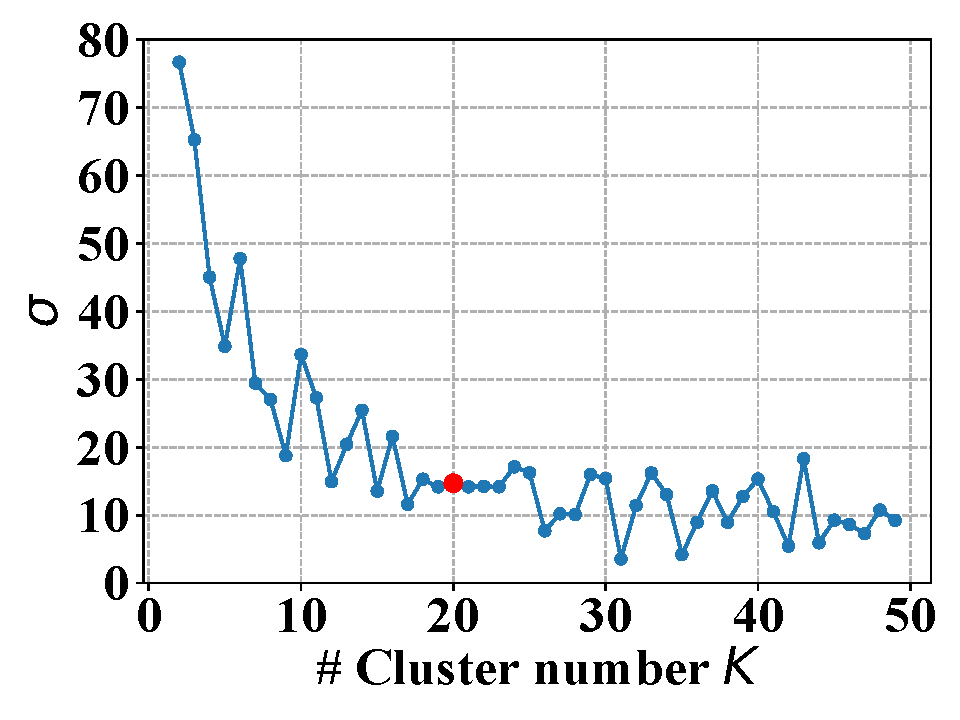
\includegraphics[width=0.23\textwidth]{figures/alphaK}
	}
	%\hspace{-0.1in}
	\subfigure[Yelp]{\label{subfig:yelpK}
		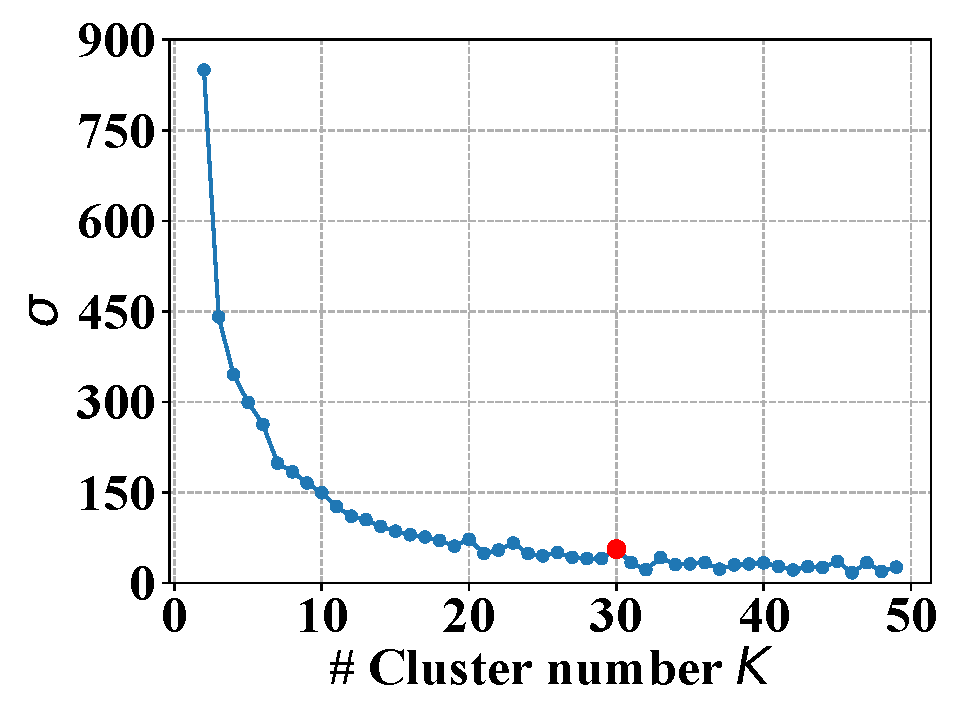
\includegraphics[width=0.23\textwidth]{figures/yelpK}
	}
	\caption{\label{fig:cluster} The correlation between the graph (cluster) number $K$ and the inertia gap $\sigma\left(K\right)$ between $K$ and $K+1$ on Alpha (a) and Yelp (b). Red point denotes the $K^*$ that achieves the best performance of \spmodel without fine-tuning.} 
\end{figure}

